\documentclass{beamer}
\usepackage{tikz}
\usepackage{lmodern}
\usepackage{movie15}
\usepackage{graphicx}
\usepackage{animate}
\graphicspath{{../tex_files/report-figures/}}
\usetheme{CambridgeUS}
\title{Sieve Estimators}
\subtitle{}


\author{N.~Joesphs, M.~Wiens, B.~Draves}
\subject{Nonparametric Statistics}

\begin{document}

\begin{frame}%B
  \titlepage
\end{frame}

\section{Introduction} 

\begin{frame}{Motivating Example} %B

\end{frame}

\begin{frame}{Outline} %B
\begin{enumerate}
\item Define \textit{Sieves Estimator}
\item Properties of the Estimator
\item Derive Smoothing Selection Algorithm
\item Simulations and Applications 
\end{enumerate}
\end{frame}

%-----------------------------------------------------------------
\begin{frame}{Sieves}%M
\begin{itemize}
\item \textit{Sieve Estimation} constructs a sequence of function spaces $\{\mathcal{F}_n\}_{n=1}^{\infty}$ such that $$\mathcal{F}_1\subset\mathcal{F}_2\subset\mathcal{F}_3\subset\ldots$$
\item Then, depending on the sample size $n$, the estimation procedure is performed over the optimal space $\mathcal{F}_{opt}$
\item Heuristically, as $n$ increases, we attain a more robust understanding of the data and should allow the modeling procedure to consider more complex functions
\end{itemize}
\end{frame}
%-----------------------------------------------------------------
\begin{frame}{Definitions}%M

\begin{enumerate}
\item \textbf{Goal}: Estimate unknown regression function for $Y = f(X)$
\item We consider the \textit{series estimators} of $f$ $$ \mathcal{F} = \Big\{g(x): g(x) = \sum_{d=0}^{D} \alpha_{d} \phi_{d}(x)\Big\}$$  where $D\to\infty$ and $n\to\infty$ \pause
\begin{itemize}
  \item $\phi_d(x)$ is the $dth$ basis function
  \item $\alpha_d$ is the corresponding coefficient  
  \end{itemize}
\item The complexity of $\mathcal{F}$ increases as $n$ increases
\end{enumerate}
\end{frame}
%-----------------------------------------------------------------
\begin{frame}%M
{Basis Functions}
\begin{enumerate}
\item Choosing basis function is analogous to choosing kernel 
\item Basis functions should represent belief about the underlying function 
\item Some popular choices include wavelets and splines and others given below 

\begin{table}[h]
\begin{center}
\begin{tabular}{|c|c|}
\hline
Basis Functions & Functional Form\\
\hline
Polynomials & $\sum_{i=0}^{d} c_d x^d$\\
Fourier &$a~cos(\pi d x) + b~sin(\pi d x)$\\
Gaussian &$\varphi^{(d)}(x)$\\
\hline
\end{tabular}
\caption{Series estimators with basis function $\phi$ for $\hat{g}(x)$}
\label{tab:basis}
\end{center}
\end{table}

\end{enumerate}
\end{frame}
%-----------------------------------------------------------------

\section{Development \& Properties}
\begin{frame}{OLS Formulation}%B
\begin{enumerate}
\item We note the similarity between the series estimator and a general linear estimator\pause 
\item Using the following matrices
$$Y = \begin{bmatrix}Y_1\\ Y_2\\\vdots\\Y_n\end{bmatrix}, P_D = \begin{bmatrix}\phi_0(x_1) & \ldots & \phi_{D}(x_1)\\\vdots & \ddots & \vdots \\\phi_0(x_n) & \ldots & \phi_{D}(x_n)\\\end{bmatrix}, \alpha = \begin{bmatrix}\alpha_0\\\alpha_1 \\\vdots\\\alpha_D\end{bmatrix}, e =\begin{bmatrix}e(x_1)\\e(x_2)\\\vdots\\e(x_n)\end{bmatrix}$$
we can write our model as $$Y = P_D\alpha + e$$\\
\item Bias and variance depend on choosing $D$ correctly
\item Note that $D$ is our smoothing parameter - analogous to the bandwidth in kernel density estimation 
\end{enumerate}
\end{frame}

%-----------------------------------------------------------------
\begin{frame}{MISE}%B
\begin{enumerate}
\item We choose our optimal dimension $D_{opt}$ by minimizing MISE 
\item We can decompose the variance of the estimate as $e(x_i) = \epsilon(x_i) + r(x_i)$
\begin{itemize}
  \item $\epsilon(x_i)$ random error around true regression function
  \item $r(x_i)$ error due to misspecification of $D$ 
\end{itemize}\pause
\item MISE can be written as $$MISE(D) = E[r^{2}(x)] + tr\Big[E[\phi(x)\phi(x)^{T}]E\left((\hat{\alpha} - \alpha)(\hat{\alpha} - \alpha)^{T}\right)\Big]$$
\item Even under the assumption of homoscedasticity $$MISE^*(D)\simeq E[r^2(x)] + \frac{\sigma^2 D}{n}$$
which is still a function of the unknown $r(x_i)$
\end{enumerate}
\end{frame}

%-----------------------------------------------------------------
\begin{frame}{Connecting MISE and PSE}%N
\begin{enumerate}
\item While MISE is infeasible, MISE is connected to PSE 
\item Let $x^{*}$ be a new data point. The sieve estimate of $x^{*}$ is given by $$y^{*} = \hat{g}(x^{*})$$ with error $e^{*}$
\item Then we can show the relation $$PSE\Big(\hat{g}(x^{*})\Big) = Var(e^{*}) + MISE\Big(\hat{g}(x)\Big)$$
\item Therefore, minimizing MISE is equivalent to minimizing PSE
\end{enumerate}
\end{frame}
%-----------------------------------------------------------------
\begin{frame}{Connecting PSE to CV}%N
\begin{enumerate}
\item Let $\tilde{e} = Y^{*} - \hat{y}^{*} = E[\tilde{e}^2]$
\item We interpret this as the expectation of a single leave-one-out squared prediction error
\item This gives rise the leave one out cross validation criterion $$CV(\hat{g}) = \frac{1}{n}\sum_{i=1}^n\tilde{e}_{i}$$ where $\tilde{e}_i = y_i - \hat{y}_{(i)}$
\item This establishes a relation between MISE, PSE, and CV \pause 
\item Hansen (2012) show that choosing $D$ based on this procedure is asymptotically equivalent to choosing $D$ based on MISE
\end{enumerate}
\end{frame}
%-----------------------------------------------------------------

\section{Applications}

\begin{frame}{Simulation Design}%N
\begin{enumerate}
\item Recall the model from HW5 given by
$$Y = \sin^3(2\pi X^3) + \epsilon$$
where
$$X \sim N(0, 1)$$ $$ \epsilon \sim N(0, .2)$$
\item Our previous solution: LLR and Kernel Regression
\item Applying polynomial sieves 
\begin{itemize}
\item $N = 150$ data points
\item From $n = 10$ to $N$ in increments of $10$, we fit polynomial series estimator with degrees of complexity varying from $1$ to $8$
\item Repeated this on $200$ separate datasets and plotted the PSE against $n$
\end{itemize}
\item \href{https://raw.githubusercontent.com/matthewrw/Sieves_Project/master/R_code/sim_gif2.gif}{Simulation Results}
\end{enumerate}
\end{frame}
%-----------------------------------------------------------------
\begin{frame}{Simulation Results}%N

\end{frame}
%-----------------------------------------------------------------
\begin{frame}{Geyser Data Application}%M
\begin{figure}[h]
    \centering
    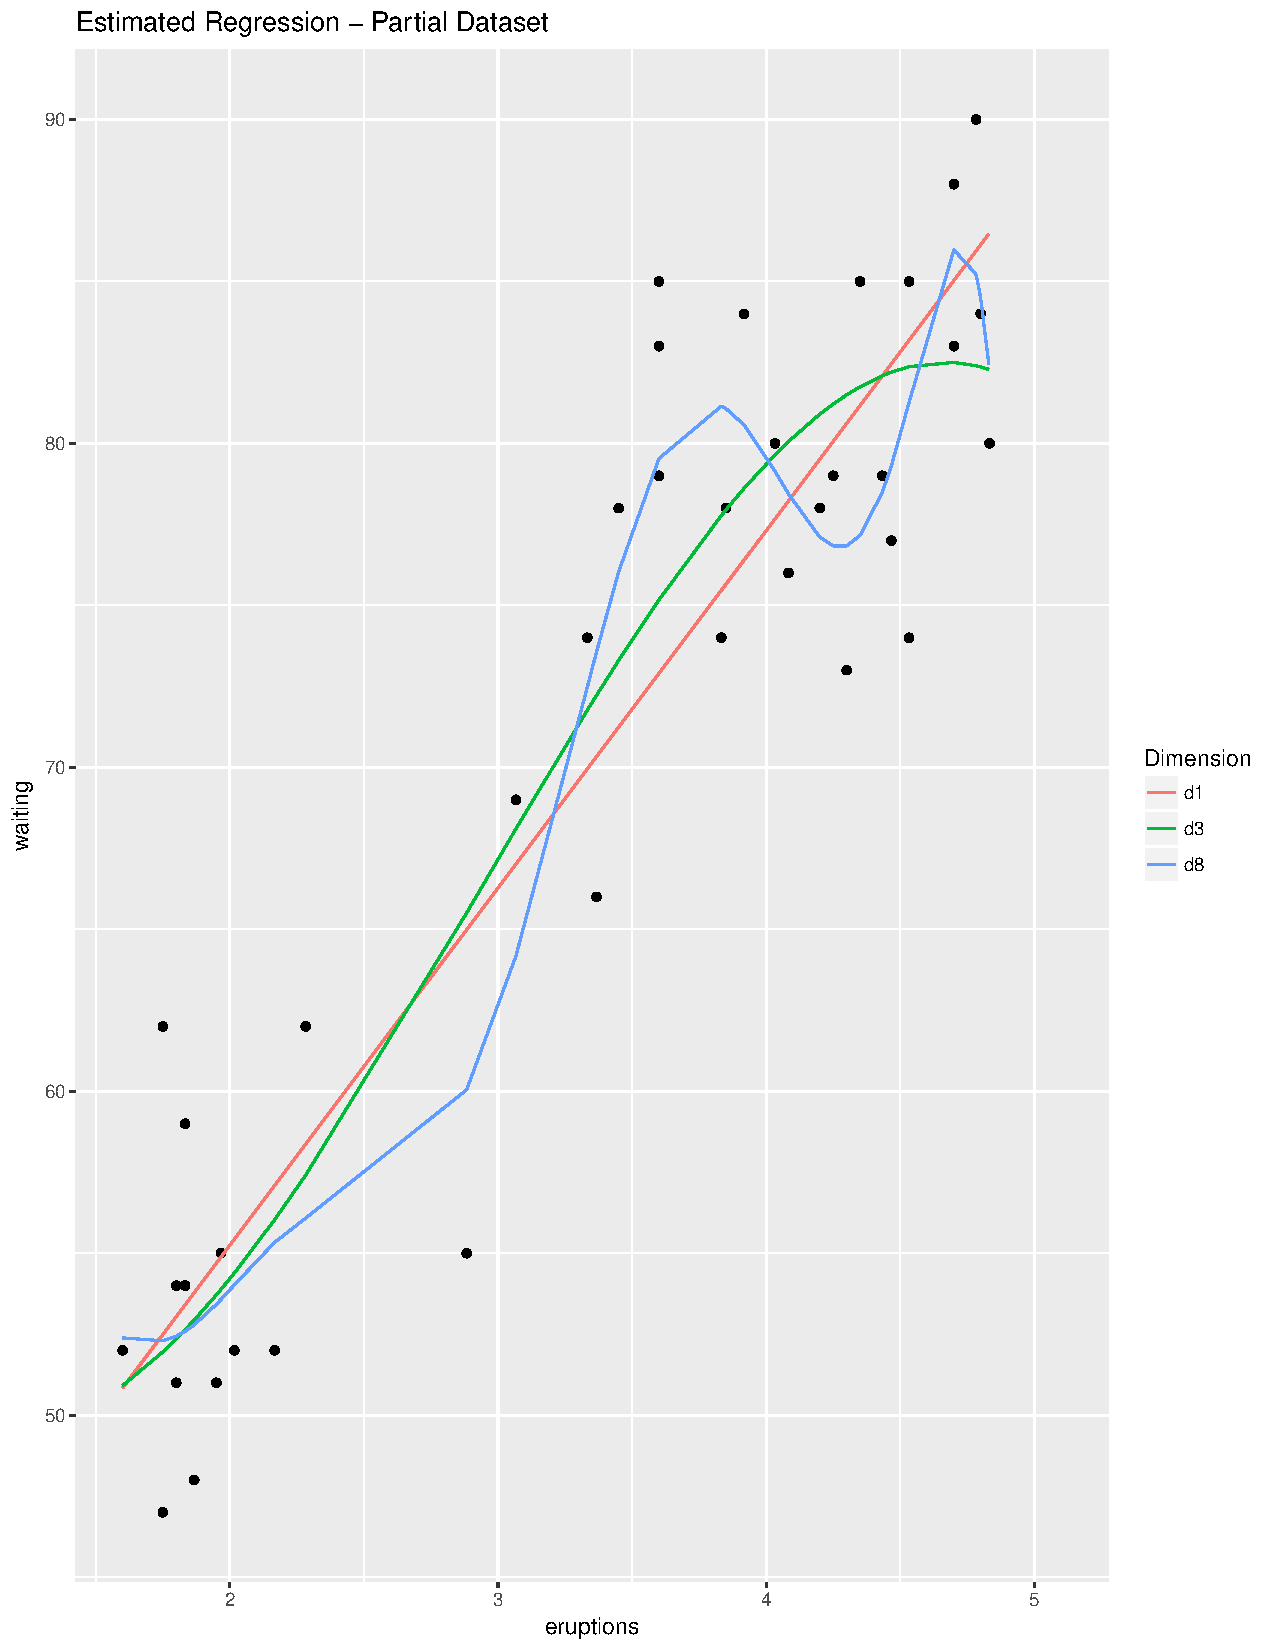
\includegraphics[width=0.45\textwidth, height = 6cm]{Geyser_Small_Data.pdf}
    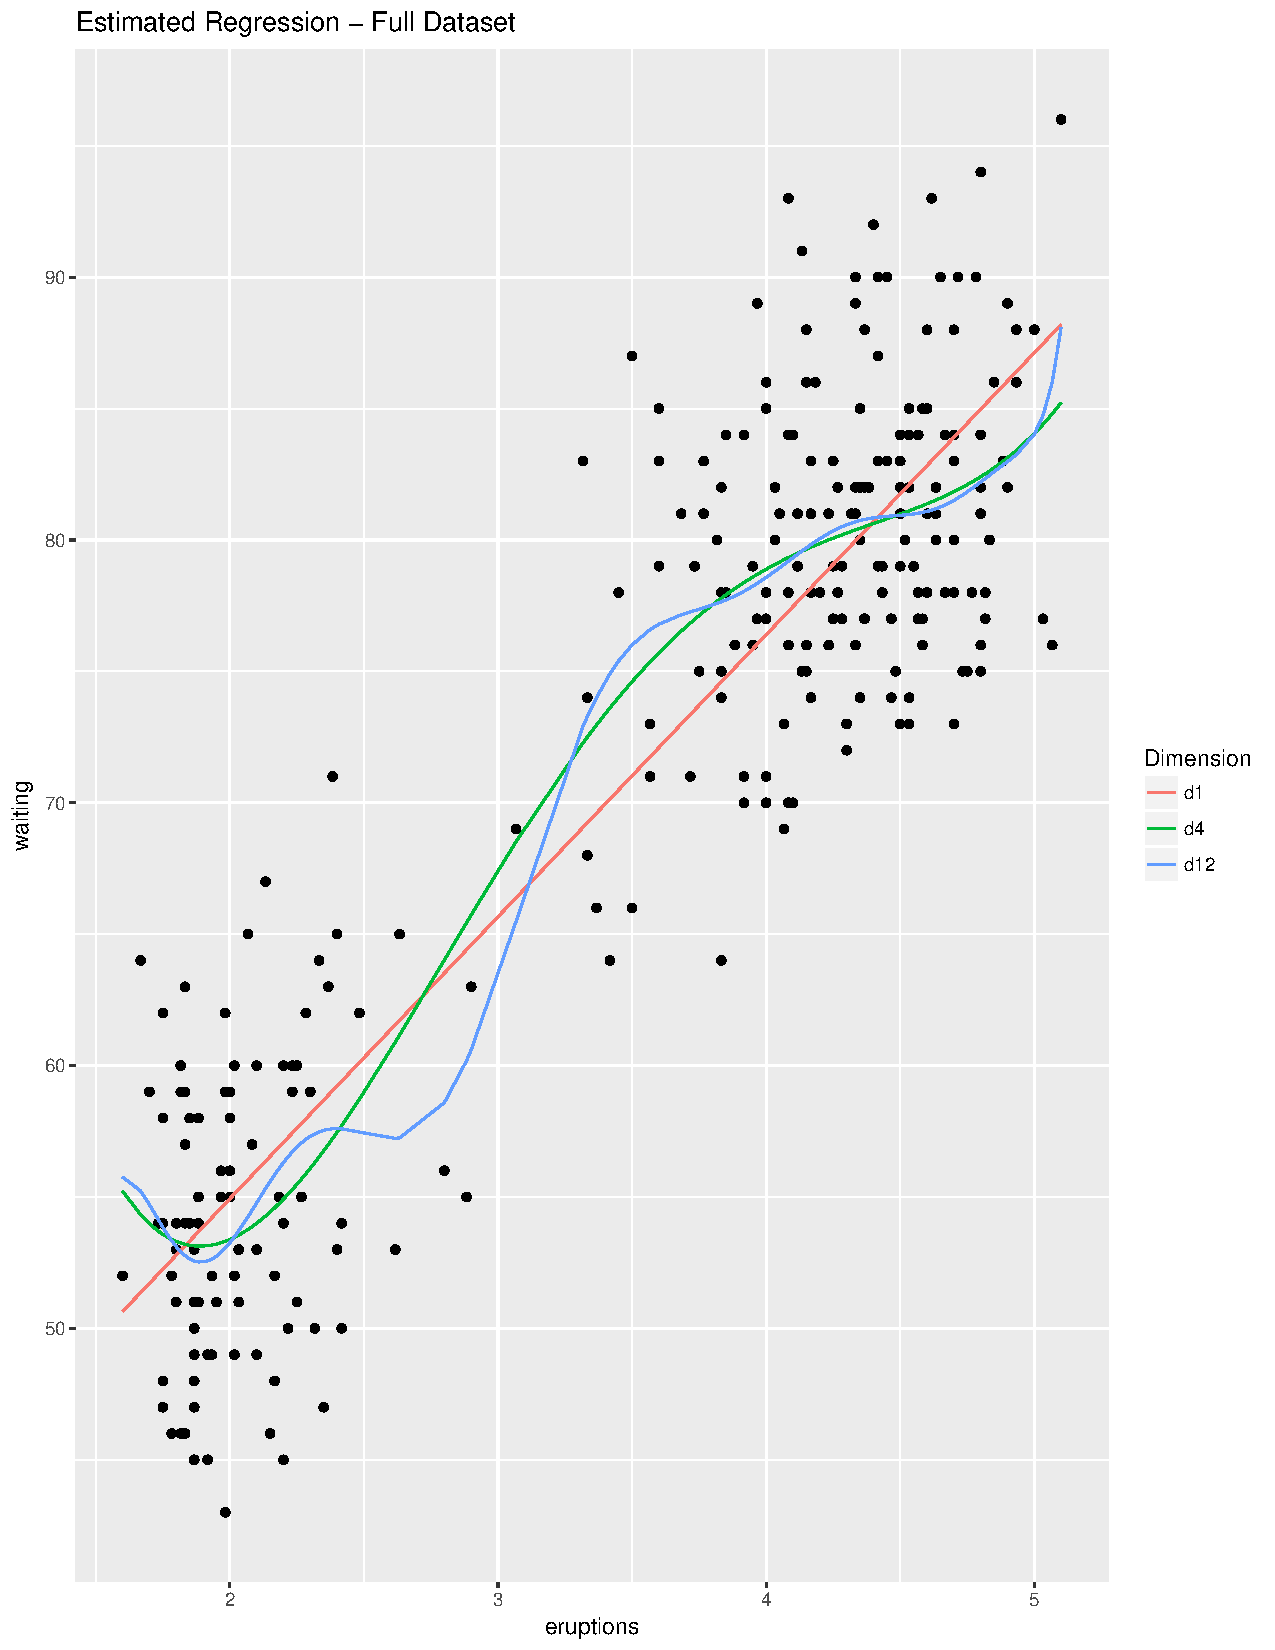
\includegraphics[width=0.45\textwidth, height = 6cm]{Geyser_Full.pdf}
    \caption{Sieves Analysis of Geyser dataset. We see that increasing our sample size leads to differing optimal models}
    \label{fig:Geyser}{}
\end{figure}
\end{frame}
%-----------------------------------------------------------------
\begin{frame}{Geyser Data Application}%M
\begin{figure}[h]
\centering
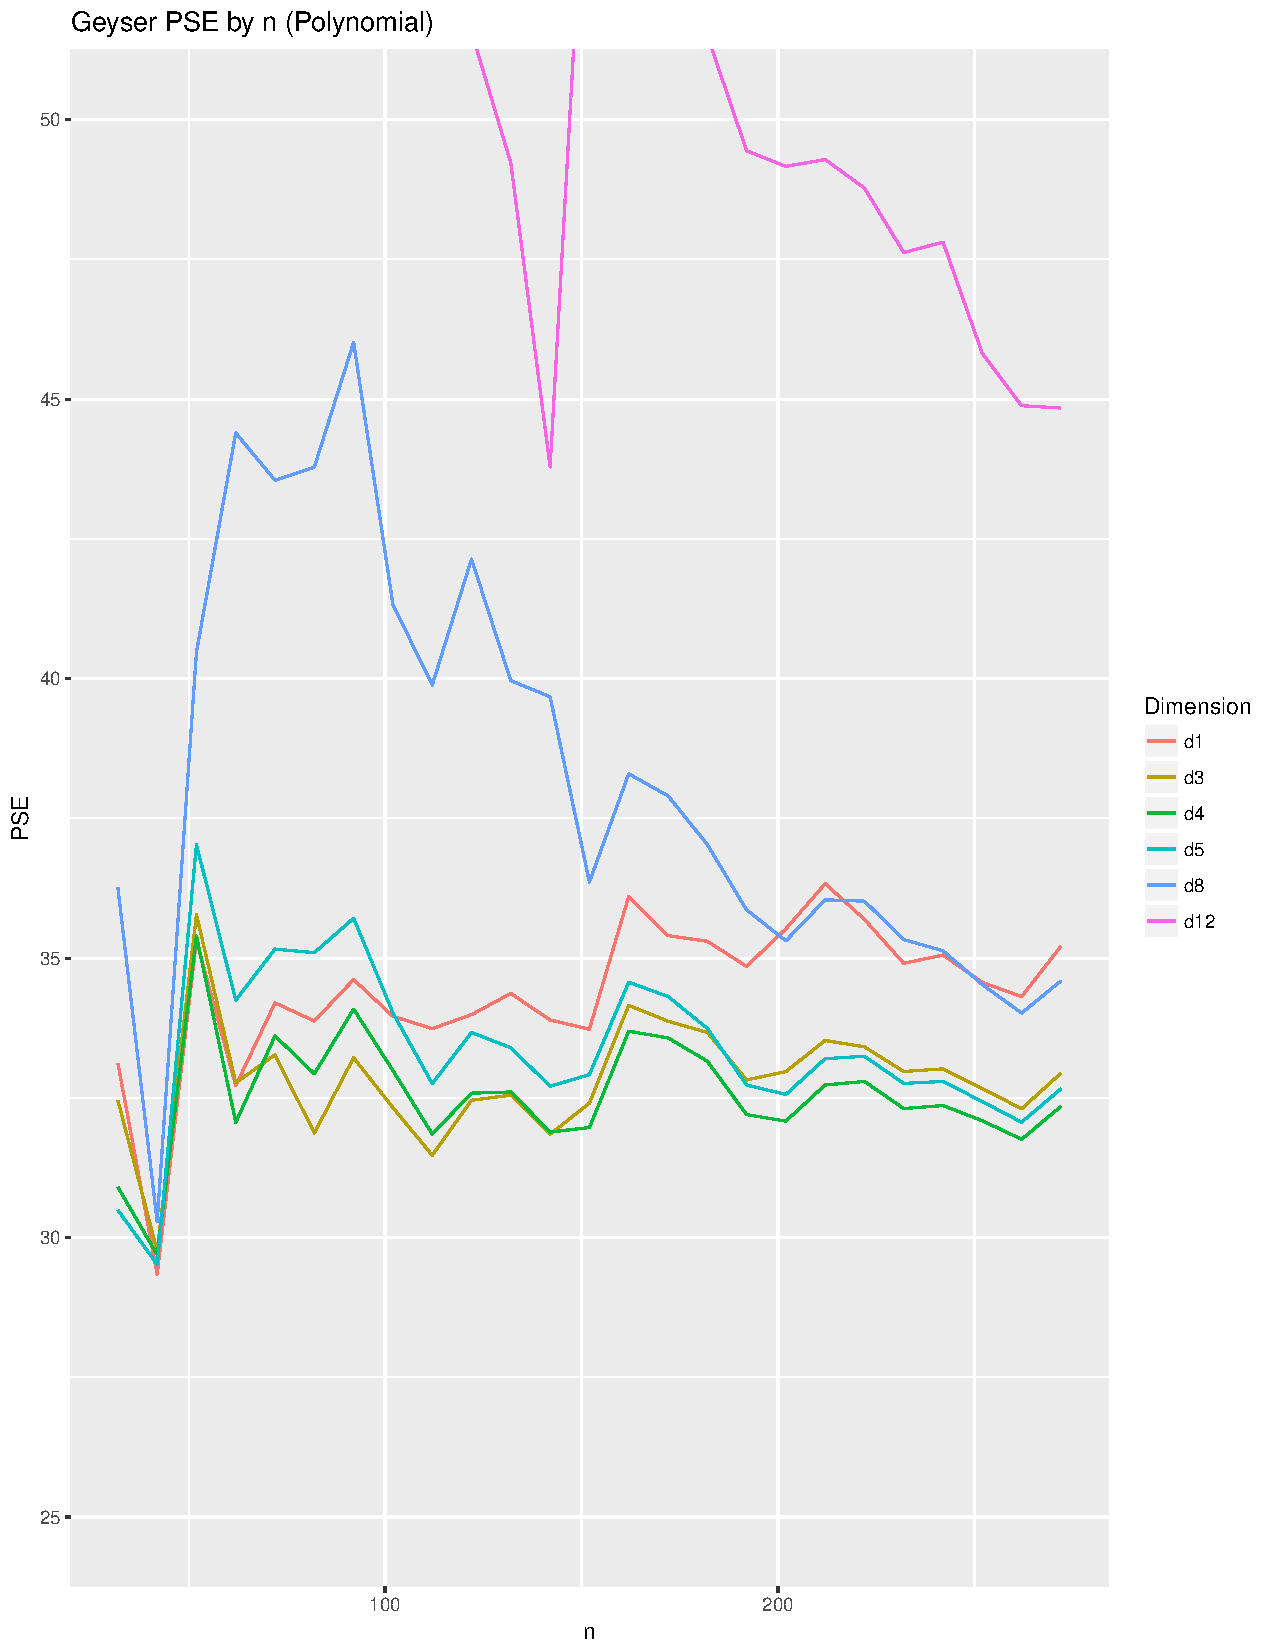
\includegraphics[width = 7cm, height = 6cm]{Geyser_PSE.pdf}
    \caption{Geyser data PSE by $n$}
    \label{fig:Geyser}{}
\end{figure}
\end{frame}
%-----------------------------------------------------------------
\begin{frame}{Sieve Estimators and Monetary Policy}%M
\begin{enumerate}
\item Sa and Portugal (2015) attempt to estimate a multi-dimensional loss function with a sieve estimator
\item The authors use a polynomial basis to estimate derivatives 
\item Based on tests for third derivative they conclude there is asymmetry in the loss function 
\item This corresponds to additional loss for low inflation (deflation) with regard to deciding policy
\end{enumerate}
\end{frame}
%-----------------------------------------------------------------
\begin{frame}{Conclusion}%B
\begin{enumerate}
\item Introduced sieves as a nonparametric dimension adaptive estimator \pause
\item Analyzed and developed for the case of polynomial series estimators in regression \pause
\item Showed a data driven process for selecting $D$\pause
\item Illustrated the estimators in simulation and real data applications \pause
\end{enumerate}
\end{frame}

\end{document}


